\section{Physical Network Service Composition}
\label{sec:physical}
Before venturing into Virtualized Network Functions, it needs to be clarified what network functions are in general, how they are implemented and composed \textit{physically}, and what the motivations are to move towards virtualizing them. 

Networks are the backbone of any modern IT infrastructure, and with the unstoppable rise of  Cloud Computing services their importance is ever increasing. This sharp rise in relevance causes the setup and operation of previously unthinkable data centers. Providing specific functioniality in such an environment has traditionally been the task of dedicated hardware that implemented services of many different domains. These include security functions that setup firewalls, scan for viruses and detect intruders but might be applied to ``...to any data plane packet processing and control plane function...''\cite{nfv_wp}. The advantage of using Application-Specific Integrated Circuits (ASICs) lies in the potential for optimization. When designing a device that serves a very specific purpose, the application scenario can be anticipated much better than with general-purpose hardware. This typically leads to lower power consumption, higher efficiency and better output, but drives up the purchasing cost. Additionally, the operational cost is also high, since acquiring, configuring, deploying and maintaining such middleboxes is often a tedious, manual-heavy task. Nevertheless, this type of \textit{physical} function delivery has historically been the primary way of building and operating networks, especially in a data center or telecommunication and internet service provider environment. This is due to the fact that there have not been production-ready, open source solutions available that could have been deployed on so-called \textit{whiteboxes}. White boxes are devices built from general-purpose hardware that are often employed in software defined networks, due to their modifiable nature. The logic was rather already integrated in the hardware, with almost no chance of customizing it.


\begin{figure}[h]
	\centering
	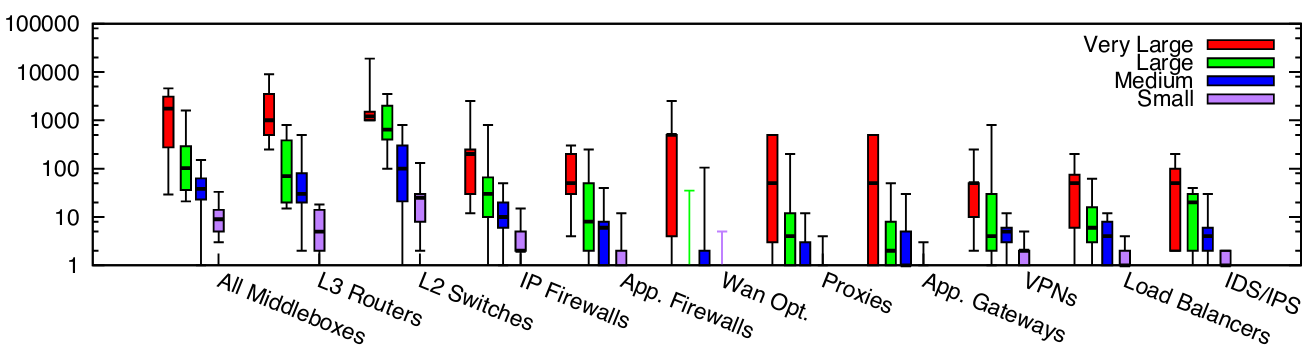
\includegraphics[width=1\linewidth]{images/middleboxesNumbers.png}
	\caption{Middlebox deployments in enterprise networks of various size (< 1k - >100k hosts). Y-axis in log scale, source \cite{sherry2016middleboxes}}
	\label{img:middleboxesNumbers}
\end{figure}

\begin{figure}[h]
	\centering
	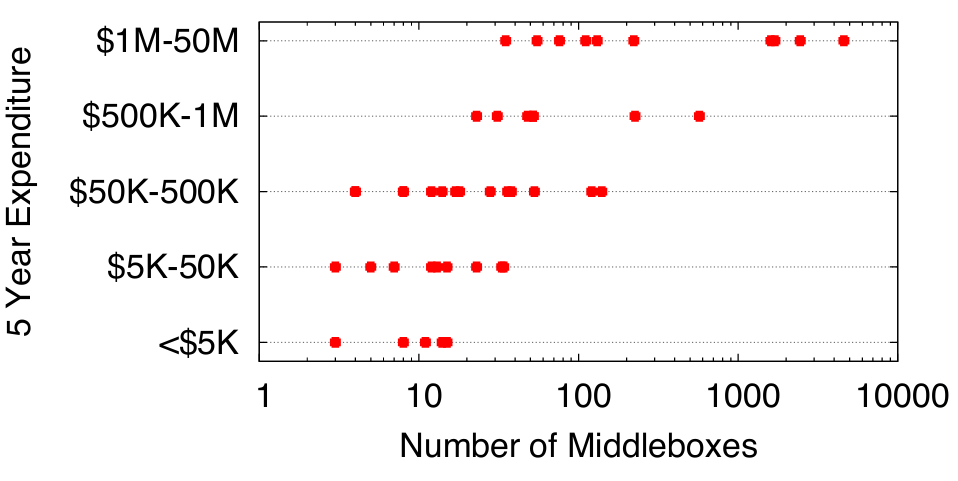
\includegraphics[width=1\linewidth]{images/middleboxesCost.png}
	\caption{Administrator-estimated spending on middlebox hardware per network \cite{sherry2016middleboxes}}
	\label{img:middleboxesCost}
\end{figure}

Figure \ref{img:middleboxesNumbers} illustrates the sheer amount of devices that are needed to guarantee the operation of enterprise networks of various size. Sherry \cite{sherry2016middleboxes} \cite{sherry2012survey}  investigated the distribution of these boxes among 57 educational and enterprise networks by surveying the operators for their experiences with the network appliances. Special focus was put on the quantity, their concerns, the cost and the ease of management. The results of this work give a good indication why this situation is unsustainable for future networks:  The number of this kind of hardware is very high. To put it into perspective, the amount of these function specific devices approaches that of fundamental hardware like L3/L2 infrastructure. The associated cost of deploying such a large number of devices can be inspected in figure \ref{img:middleboxesCost} and indicates that investment cost is skyrocketing. Naturally, this might not be a problem for small companies that use a little amount of these devices. However, Cloud and Internet Service Providers rely on building, maintaining and reorganizing enormous computer networks and thus are driving forces behind alternative concepts in this domain \cite{sherry2016middleboxes} \cite{sherry2012survey}.

\section{Network Virtualization}
\label{sec:networkV}
Breaking up this vertical integration that results in tedious and labor heavy network orchestration will only gain importance with higher complexity and higher demand of the networks that are being built. Motivating the search for alternatives are various factors, like growing cloud data centers, the implementation of 5G and all the use cases that come with it. As an example of such a demanding service provided in the cloud is \textit{Google Stadia}, a streaming service for video games. A very interesting scenario since low latency and high bandwidth is of utmost importance and needs to be guaranteed. Additionally, the provisioning and deployment of resources needs to happen instantly. This project might be paving the way for more ``serious'' applications like taking over functionality in autonomous driving for instance. 

Another relevant use case scenario includes the possibility of implementing a \textit{tactile internet} that allows to put distant environments in someone's reach. Such a scenario where this might be needed is remote surgery, where a surgeon would use a remote controlled robot to perform a procedure in a distant place. In order for this to work, unforeseen latency, fault-tolerance and reliability has to be ensured. Fulfilling such demanding requirements is only possible if the supporting network is highly flexible and can guarantee not only continuous connectivity, but also high performance. 

The previously described challenges can only be overcome when the need for the manual configuration and deployment that takes place on a box-to-box basis of function-specific hardware can be eliminated. The answer to this challenge is virtualization of the functionality in question which makes it both more configurable and highly maintainable. In order to take advantage of this virtualization, though, the encompassing network needs to support feasible possibilities to manage the virtual instances of network functions. Without a degree of automation and a centralized, programmatic approach, there would not be a huge benefit of going from physical to virtual. Software Defined Networking is ideal and often goes hand in hand with using these cutting edge technologies.

Aside from the performance standpoint, this is also an ideal way to reduce cost significantly. This is due to multiple factors, such as the high purchasing cost of the middleboxes. Additionally, the devices often provide vendor-specific means for configuration which entails high administrative and operational cost causing a lot of personnel training and the need for special spare parts.  The investment into retraining the staff that has to work with such devices can even influence the decision making process since without the expertise, smooth operations of the network are questionable. 

Once it is time to update or upgrade the parts of the network that provide certain functionality, another advantage becomes quickly apparent: With purpose-specific hardware, the only way to to get the newest features is to replace the outdated hardware with the newer model. And if more instances of the functionality is needed, acquiring more devices is the only choice to allow for scalability or provide fault tolerance via replication. Additionally, when a new appliance comes out, until it has been successfully deployed, it often already is outdated. With softwarized instances of this functionality, proven software development practices can easily be applied in order to mitigate this problem. Updates, upgrades or in the worst case, reinstallation of a program guarantee an easy path to deploy the newest functionality. Replication of a service can also be done much easier and quicker by means of virtualization. Spinning up an additional virtual machine, or in later scenarios another container, is more practical than relying upon physical boxes. 

As already mentioned, virtualization and providing the network functionality as software packages that can run on general-purpose hardware anywhere is the core promise of network virtualization. This principle has caused a paradigm shift in recent years in networking that has lead to many projects and software solutions. In the following sections Software Defined Networking (SDN), Network Function Virtualization (NFV) and Virtualized Network Functions (VNF) will be briefly introduced as the main driving forces and central ideas behind the virtualization efforts. 


\subsection{Software Defined Networking}
\label{sec:sdn}
The unobstructed operation of highly distributed applications and the offer of services depends highly on mitigating faults in the network and the appropriate reaction to fluctuating load. In traditional networks, there is hardly any support to implement automatic policy change as a reaction to events like spikes in load or the reconfiguration when faults occur in the system \cite{kreutz2015software}. When faced with such situations, ''[\dots] every single hardware instance [\dots]`` \cite{grossmann2013auto} is in need for manipulation to realize the desired change.  The need for manual intervention is responsible for immense risk regarding service interruption. The high complexity associated with this kind of networks introduces a lot of inertia and in the worst case ends in a state known as \textit{ossification} \cite{nunes2014survey}. Providing network abstractions as a service is unthinkable in such a scenario, since quick, automatic and seamless planning, provisioning and reliable configuration can not be guaranteed.

\begin{figure}[h]
	\centering
	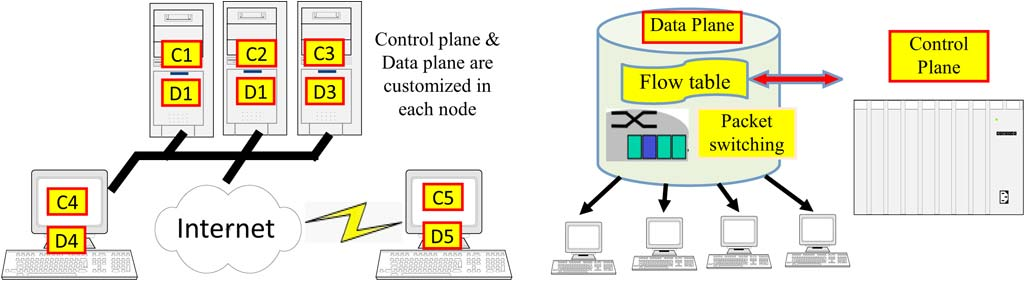
\includegraphics[width=0.48\textwidth]{images/sdn.png}
	\caption{Comparison between traditional (left) and Software-defined Networks (right), source \cite{li2015software}}
	\label{img:sdn}
\end{figure}

%PNF to NFV
Breaking up the rigidity is of utmost importance to building more flexible and cheaper networks that can  meet the demands of the future. Software Defined Networking is the technology of choice when there is a need for programmable networks. The core premise is the separation of the so-called control- and data planes, which are traditionally vertically integrated in switching devices. The logic that controls the packet forwarding and orchestration of the data flow is located inside the devices, just as well as the data structure that stores the rules for forwarding. This disallows for external manipulation while introducing the need for relying upon the vendor specific way of configuration and thus ''[\dots]  reducing flexibility and hindering innovation [\dots]``\cite{kreutz2015software}.

In SDN the control layer is being externalized and abstracted from all the switching infrastructure into an external controller instance that provides multiple means of organizing and configuring the traffic flow in the managed devices. Figure \ref{img:sdn} provides a comparison between the two concepts, where the traditional, vertically integrated switches can be seen on the left. Each device contains its own logic that controls the incoming and outgoing packets. Additionally, a middlebox that might provide the functionality of a firewall, is closely attached to the middlebox on the right circumventing the problem that the switches and routers only provide limited configuration. Problems arising from the reliance on such middleboxes have been discussed in section \ref{sec:physical}.  On the right hand side, the control plane has been externalized from the three nodes into a centralized software control. The solid edges represent data flow, while the dashed lines show the control and monitoring traffic that takes place between the controller and the boxes under its domain.

\begin{figure}[h]
	\centering
	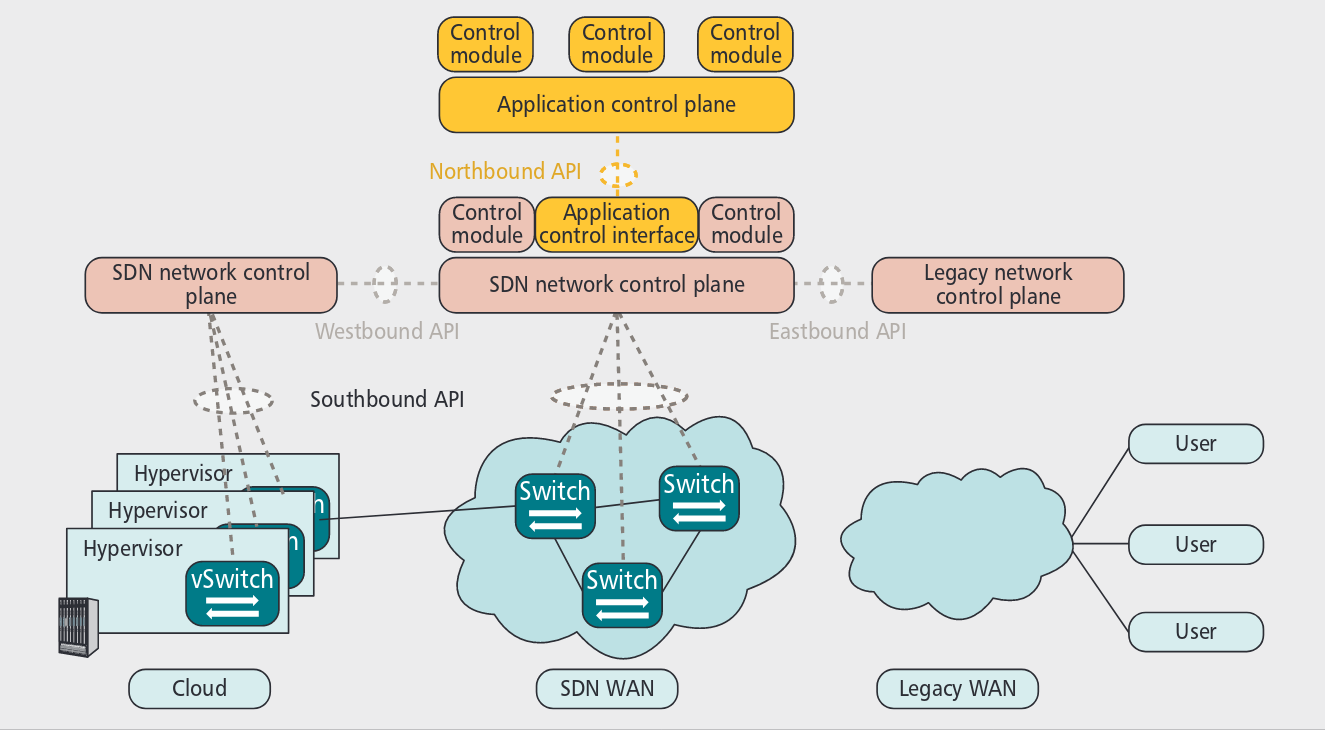
\includegraphics[width=0.49\textwidth]{images/sdnAPIs.png}
	\caption{The different elements of the SDN architecture, connected via several APIs. The northbound for application communication, westbound for inter controller synchronization, eastbound for legacy networks and southbound for device communication, source \cite{jarschel2014interfaces}}
	\label{img:sdnAPIs}
\end{figure}

In this kind of architecture, there are multiple, very important advantages: Policies can be defined and enforced on all devices almost instantly, without the need for cumbersome, vendor-specific configuration effort. The boxes no longer need to implement any control logic, and are reduced to programmable forwarding switches that only need to support the communication with an SDN controller. Visualization and monitoring of the devices is taken care of by the same program, facilitating the operation and problem solving. A common protocol provides the basis for communication and the sending of commands between the devices and the controller that can run on any kind of hardware. Finally, such controllers often provide an API to write custom applications, allowing for very fine-grained customization that circumvents the need to wait for a hardware vendor to implement and roll-out a new feature. As a side note, since this figure suggests the controller constitutes a single point-of-failure, many controllers support the concept of clustering. Deploying multiple instances mitigates the risks when one is failing and can be used for a smooth rollout once a new version is available.  

Programming of the devices throughout the network works over a standardized protocol that allows to manipulate the data or forwarding plane of each device. The Open Network Foundation (ONF) develops and manages \textit{OpenFlow}, a protocol that was originally proposed so that researchers could ''[\dots] run experiments on heterogeneous switches in a uniform way at line-rate and with high port-density;``\cite{mckeown2008openflow}. As the technology matured, it has become one of the best known enabling technology for SDN. Generally speaking, a software controller can support multiple of these protocols via its Southbound API making it even more flexible. The choice of such a protocol depends on what protocols the managed devices support mainly. 

With OpenFlow for instance, a controller can manipulate a so-called \textit{flow table } for each switch. This table represents the packet forwarding rules that determine the handling of an incoming packet. If no rule applies, the standard behavior is to send the packet for further analysis to the controller, which will then inspect the packet. This is where the power of SDN comes to play, since an in-depth analysis of the packet can reveal useful information that can be used to determine how to deal with it. The packet can be ignored, it can be forwarded and new rules and routes can be established, or a custom application could trigger an alarm or even trigger the deployment of a new service or network function that might be overloaded or missing. A considerable advantage is that the setup of the traffic rules needed to ensure connectivity, can be done at this place where all relevant information is available. When deploying a new network function on a compute node, it can be instantly ensured that it is connected correctly to its environment. Extending the logic via additional applications is done via the Northbound API. The Westbound API is needed to provide the communication between multiple instance of the controller software. These might be needed to provide fault tolerance or a logical separation of the devices. The last API is located Eastbound and provides a point of communication with legacy networks and downward compatibility. All these different elements that make up an SDN controller can be inspected in Figure \ref{img:sdnAPIs}.

East and Westbound APIs are not part of all architecture specifications and present in Sezer \textit{et al.} \cite{sezer2013we} for instance. The authors reserve the west- and eastbound APIs for inter cluster communication of multiple controller instances. \cite{hu2014survey} \cite{jarschel2014interfaces} \cite{nunes2014survey} \cite{sezer2013we} \cite{shin2012software} \cite{jammal2014software}.

\subsection{NFV}
\begin{comment}
 \begin{description}
 	\item often monolithic, scaling coarse grained, whole vnf needs to be replicated
 	\item some functions repeatedly (unnecessarily) called in sercice function chains
 	\item vnf as a bumb in the wire
 	\item \cite{chowdhury2019re}
 \end{description}
\end{comment}

\subsubsection{NFV SDN relationship}
% NFV SDN relationship
Putting a controller in charge of the switching infrastructure in a network allows for flexibility and network programmability. This concept is complementary to that of providing functions in a virtualized manner that have previously been running on purpose-specific hardware. These two concepts do not necessitate each other, since they can be deployed and used independently. Nevertheless, they are in support of the same idea: Facilitating the network setup, operation and upgrade via the means of virtualization and softwarization. Their relationship is so close, that even the white paper for NFVs dedicates a subsection to this. Making use of both concepts can proof mutually beneficent since ''[\dots] approaches relying on the separation of the control and data forwarding planes as proposed by SDN can enhance performance, simplify compatibility with existing deployments, and facilitate operation and maintenance procedures. Network Functions Virtualization is able to support SDN by providing the infrastructure upon which the SDN software can run`` \cite{nfv_wp}. 


% NFVs 
\subsubsection{PNF to VNF}
After SDN has introduced a paradigm which promises flexible reconfiguration of a network, the idea of running network functions on general purpose hardware in virtualized environments in the form of \textit{NFV} has taken shape. Leaving behing ASIC boxes and orienting oneself towards software solutions lie at the heart of this technique. ETSI, the European Telecommunications Standards Institute, founded by multiple telecommunications providers and operators, has put forward a white paper in 2012 defining critical aspects to this new technology \cite{nfv_wp}. After this had been published, the proposal has gained a lot of momentum and implementations that allow to make use of this new technology have been put forward, which are taken into consideration when planning and building networks ever since \cite{ordonez2017network}.

\begin{figure}[h]
	\centering
	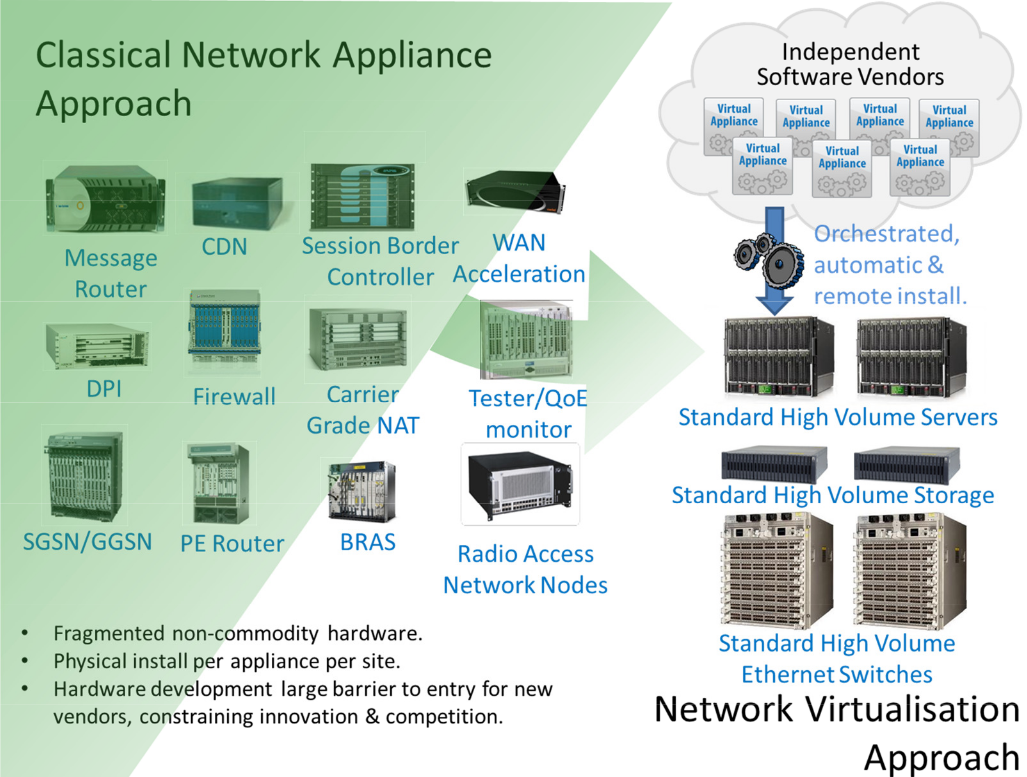
\includegraphics[width=0.5\textwidth]{images/nfv.png}
	\caption{From ASICs, to virtual appliances, source \cite{nfv_wp}}
	\label{img:nfv_wp}
\end{figure}

Figure \ref{img:nfv_wp} visualizes why SDN and NFV are often described as a \textit{paradigm shift}. The network landscape and physical composition can change considerably as the shift from left to right indicates. The left side shows the classical approach, relying on a multitude of heterogeneous, vendor-specific and non-standardized devices that are built for one specific purpose. These \textit{black boxes} are scattered all over and need to be manually configured in order to work. Implementing their functionality in pure software and packaging it into artifacts that can be executed on standard devices present throughout the network, provides an unprecedented liberty in composing and orchestrating the functionalities desired be found inside  network. Decoupling the actual application logic from their physical surroundings also favors the emergence of a broader ecosystem where such programs are developed and shared, rendering this concept even more appealing.

\subsubsection{NFV Architecture}
Virtual appliances can either be developed or procured from emerging software ecosystems. As a part of this vision, an orchestrator platform should take care of automatic procedures like fetching and installing it onto (virtual) appliances present in the network. The configuration for the packet flow then can be done via SDN (not part of the figure) which shows why these two concepts go hand in hand. 

A conceptual architecture overview is given in Figure \ref{img:nfv_ref_arch}, where several layers are combined to build a reliable and functional system. The bottom summarizes the physical hardware resources available providing different basic functionalities like \textit{compute, storage} and \textit{network}.  By exploiting the available infrastructure, a virtualization layer provides an abstraction that can be used to easier define and provide access to a required set of resources and schedule their provisioning. Predefined and runnable VNFs can subsequently be executed on the abstracted virtualized compute, storage and network devices. The systems that have been built in recent years often use virtual machines to bundle the functionality inside an artifact that can be executed almost anywhere. In order to fulfill the vision of network function virtualization and realize its full potential, automation is key. This is part of the NFV orchestrator's job, that can be fed service deployment requirements and thus reserve the resources needed and deploy the function.

\begin{figure}[H]
	\centering
	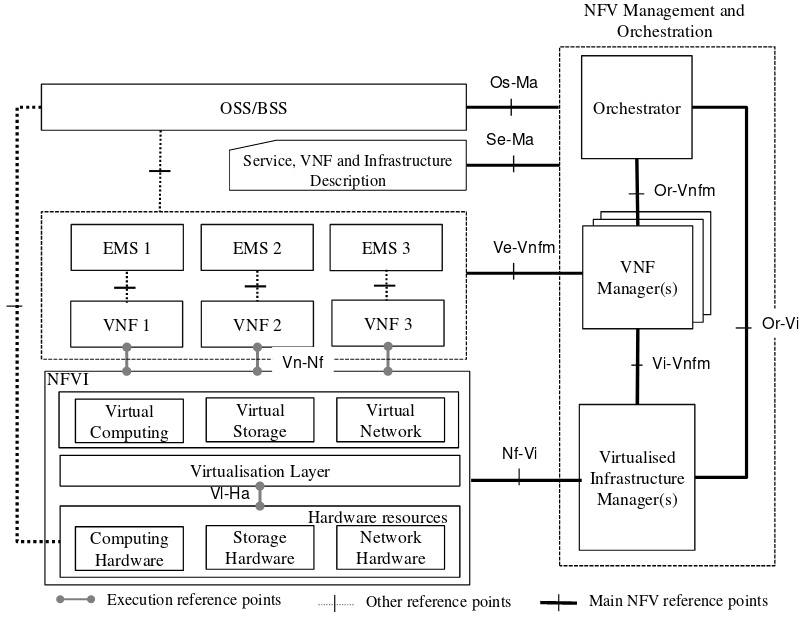
\includegraphics[width=1\linewidth]{images/nfv_ref_arch.png}
	\caption{Reference NFV architecture \cite{etsi1etsi}}
	\label{img:nfv_ref_arch}
\end{figure}

In order to ensure that virtual machines are started and stopped as needed, so that there is a platform for the VNFs to run on, there is another entity needed, namely the Virtualized Infrastructure Manager (VIM). Its responsibilities are focused on mapping the resource needs of the VNFs to specific VMs. The manager has therefore to be in charge of the underlying software that can realize such an infrastructure, including for instance hypervisors, and also the resources needed such as compute, storage and network. Allocating resources for function deployment falls also under its domain by instantiating virtual machines onto hypervisors. After the initial setup, it should take care of allocating additional resources to VMs and further optimizing their operation. This is also the place for providing an insight into operations for analyzing the performance and realize outward visibility especially for monitoring and optimizing the services. 
The VIM is part of the NFV Management and Orchestration (MANO) part of the overall architecture, located to the bottom right. The part under its control and management is the Network Function Virtualization Infrastructure (NFVI) that is the component running the actual functions that can be placed inside compute nodes all around the network \cite{nfv_etsi}. 

\subsubsection{Service Chaining}
% Service chaining
Often these functions are chained together in a process called \textit{Service Function Chaining} (SFC as defined in IETF RFC7498) to provide more complex services. Doing this with physical network functions requires manual intervention to setup such a chain. Naturally this such a process is prone to errors and results in static structures that are not easily moved or replicated \cite{luizelli2017actual}. NFVs  however provide the technological basis to compose such a complex service from heterogeneous and distributed functions. Figure \ref{img:nfv_forward} serves to illustrate an end-to-end (E2E) communication path along which the packets are being processed at multiple points. The continuous line represents the physical connection of the elements, connecting the two endpoints via NFVI Points of Presence (PoP). These NFVIs abstract from their resources with the help of virtualization and provide the environment the capability to deploy and operate network functions. The virtual networking resources are used to interconnect the different nodes to guarantee interconnection.  A service chain can be described by a forwarding graph, and the single elements can either be network functions or forwarding graphs, which allows for nested elements. Each forwarding graph is embedded inside a box of dotted lines and is interconnected via logical links, represented with dashed lines. These constitute an interface that needs to be exposed by each element in order to be able to flexibly compose a complex network service. As can be inferred from figure \ref{img:nfv_forward}, the single elements do not need to be located in one physical location, but can rather be spread across multiple domains and are supposed to also work together in a multi-vendor environment. On the one hand this opens endless possibilities and freedom when it comes to providing end-to-end services in a flexible, scalable and highly reactive manner. On the other hand this has sparked a new field of research of its own which focuses on the question of appropriate and sensible VNF deployment, especially when considering their role in network services \cite{place1} \cite{place2} \cite{place3}. This problem is so complex, that machine learning algorithms are being applied to achieve the desired results \cite{placeml1} \cite{placeml2}.  The inner workings of such an E2E service are often transparent, but some introspective has to be given, for example specified constraints that need to be fulfilled in order to assess whether the performance is acceptable for the specific use case. Some applications for instance are more latency sensitive than others, and thus require guarantees of the maximal latency of a service chain. Another example might be regulatory, where data privacy restrictions prohibit user data from being stored and/or processed outside a country's boundaries. 

\begin{figure}[h]
	\centering
	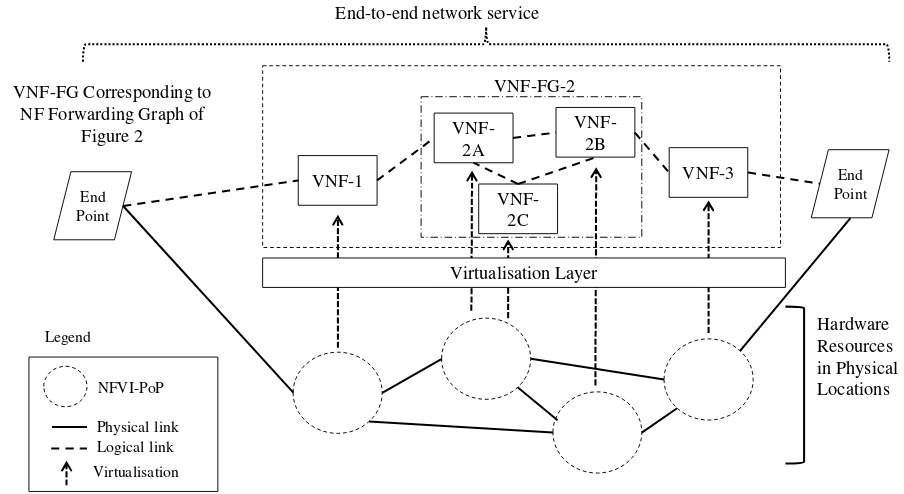
\includegraphics[width=0.49\textwidth]{images/nfv_forwarding.png}
	\caption{NFV forwarding to establish end-to-end connections \cite{ etsi1etsi}}
	\label{img:nfv_forward}
\end{figure}

\subsubsection{Motivating Use Case: EPC Virtualization}
At this point it seems appropriate to present a motivating use case where the previously discussed technologies can be demonstrated and which hopefully serves to highlight the inherent advantages. In 4G networks, one of the components is the so-called Evolved Packet Core or EPC. This part of the network is designed to provide the core network infrastructure and has its origins in GSM from where it was continuously upgraded. The breaking change introduced in 4G was the reliance upon Internet Protocol (IP) as the basic protocol to provide all services. 

\begin{figure}[h]
	\centering
	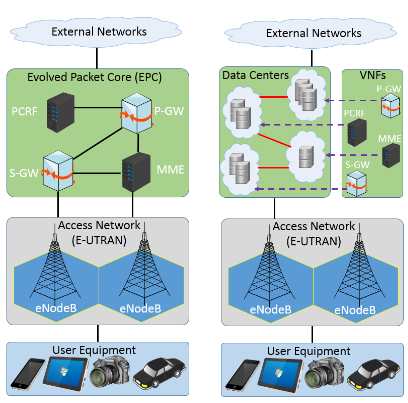
\includegraphics[width=0.5\textwidth]{images/epc_virt.png}
	\caption{Virtualization of the Evolved Packet Core \cite{mijumbi2016network}}
	\label{img:epc_virt}
\end{figure}

Figure \ref{img:epc_virt} on the left side shows how the several components of the EPC are realized with physical middleboxes and puts it into the perspective of a 4G network. . The first component of the EPC is the Policy and Charging Rules Function Server, whose main function is to take care of the service policy and Quality of Service information on a per-user basis. Establishing connection to external networks is the purpose of the Packet Data Network Gateway, connected with the Serving Gateway. The Mobility Management Entity offers control features with regard to the user equipment which is in most cases not stationary and needs to be able to connect and authenticate in a radio network environment. The physical connection of user equipment (bottom) is being established in a 4G network over the eNodeB base stations that use standardized radio frequencies.
The scenario to the right shows how this architecture can be realized when dropping expensive, hard to manage vendor-specific black boxes and rather providing the functionality of the components in a virtualized manner. Scaling and replication can be done via multiple deployments of the same VNF on general purpose hardware found in the supporting data centers inside compute nodes. The possibilities at this point are manifold, the Infrastructure as a Service (IaaS) cloud service model for instance allows to rent virtual machines in public clouds, which can complement the private cloud capabilities. 

In comparison with the traditional setup, scaling, updating and many other critical operations can now be performed in a much more economical manner. If load spikes hit the system, deploying new VM instances should take care of the incoming, additional traffic. The overall cost sinks, since only the service needed has to be payed, instead of having to purchase additional function specific devices in case of increased demand. Although this technology is becoming more and more obsolete with the oncoming fifth generation networks, this example is still highly relevant. Backwards compatibility with legacy systems will have to be ensured once 5G is the dominating technology, and what better way to flexibly do this via the means of virtualization? \cite{4g} \cite{mijumbi2016network}. 

Figure \ref{img:epc_virt} shows how a forwarding graph that uses virtualization to realize mobile Internet services would look like. In its basic layout, it is very reminiscent fo figure \ref{img:nfv_forward} both in the vertical, as well as horizontal direction. The abstraction from the physical layer is apparent as well as the decoupling of the elements' functionality. The different paths originating from the device what else is possible: providing finely grained end-to-end customized services, as opposed to traditional networks where specific features could only be (de-)activated on the whole network  \cite{abdelwahab2016network}.

\begin{figure}[h]
	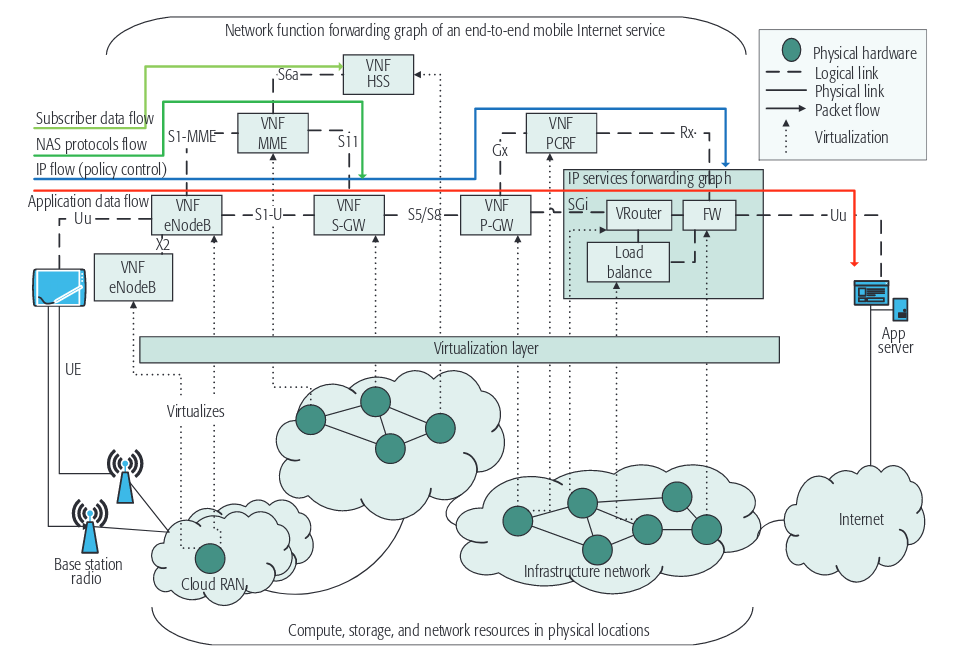
\includegraphics[width=1\linewidth]{images/mobileInternetServices.png}
	\caption{Mobile Internet service \cite{abdelwahab2016network}}
	\label{img:mobile}
\end{figure}



\subsubsection{5G Network Requirements}
As 5G deployment has already started in various locations and can be considered a disruptive technology, its importance in the context of network softwarization shall briefly be explored in the following. In 2017 ETSI published a white paper outlining the most important aspects of NFV in the context of fith generation networks, from the network operators' perspective. The vision of 5G certainly is not limited to ``just'' higher bandwidth in the up- /download  direction and lower latency. These advancements are one important element and contribute to a broader vision of  building a true, next generation network that is characterized by ``[\dots] agile resilient converged fixed/mobile networks based on NFV and SDN technologies and capable of supporting network functions and applications encompassing different domains, including serving remote areas and inside buildings'' \cite{nfv5g}. Building on this vision, new and previously unrealistic use cases and business applications can be designed upon the promise of the highly flexible and high-performance characteristics of this new network. In order to realize services complex network services, several technologies need to be taken advantage of. 

%Guaranteeing low latency for instance is a combination of multiple efforts 
First, Network slicing has been identified as a central feature of 5G, heavily relying upon NFVs and other softwarization efforts to be implemented. Network slicing can be understood as the realization of the Network as a service paradigm, where a slice consolidates a subset of the underlying resources in order to provide a custom tailed segment of the network. The components of a slice range from computing, storage and networking resources, often realized with VNFs and for traffic organization SDN and VNF Management and Orchestration elements such as control, management, orchestration and service planes. This service models allows the usage of the network by multiple tenants and each can be shaped by to one's exact needs by varying parameters.
 
Second, and this will be discussed later in more detail, are the Cloud-native Network Functions (CNF).  Virtualization has been the de-facto standard for the definition, deployment and operation of VNFs since their definition. The transformation from PNFs to VNFs has often been simplistic, meaning that the functionality contained in the physical boxes, has just been replicated in a virtual machine. This makes the transition easier, since it is an incremental step, but to further exploit the benefits VNFs can provide, especially in 5G, more agile and lightweight approaches have to be explored. 

Third stands the end-to-end service management that is closely related to network slicing. A new technology claims high investment to setup and is only justified if there is a realistic promise of new business prospects and models. Providing custom network services that are located between the two end points of communication as a service is essential to 5G networks. This simple sounding principle is extremely complex in an operational and management sense. When customers compile their own service from available components, these elements need to be reserved, provisioned, monitored and billed. Providing means to manage these services is a significant effort, that needs to take into consideration many aspects like lifecycle management, monitoring and debugging and many more, always increasing the complexity. 

Lastly, the laws of nature prohibit that for certain scenarios with strict latency requirements, the length of the service function chain exceeds a specific distance. If an application, for instance augmented or virtual reality or tactile internet like remote surgery, are being designed, they will postulate strict latency requirements that will require a round trip time of under 2ms. Light travels approximately 300km in 1ms, excluding refraction and reflection.  This severely limits the radius a network service can effectively be used. Since not all functions are required for a specific use case, splitting them up and allowing for a highly distributed placement along the lines of microservices might solve this problem. In reality, this can be realized with smaller, but numerous data centers that are closer to the users, thus lowering the distances needed to travel. This is known as edge computing in general or fog computing as defined by Cisco. Naturally, breaking up big data centers and deploying smaller ones where needed necessitates first the decoupling of the functionality from the underlying hardware, and second high automation. This ensures a significant reduce in setup and operational costs and makes the new use cases potentially profitable \cite{ordonez2017network} \cite{nfv5g} \cite{alexgalis2018multi} \cite{alexgalis2017analysis} \cite{cn5gvnf} \cite{de2019network} \cite{abdelwahab2016network} \cite{condoluci2018softwarization} \cite{nfv_wp} \cite{nfv_etsi}. 

All in all the growing capabilities of the fifth generation network can only be efficiently made use of and marketed, if the infrastructure is flexible enough to allow for this new level of demand towards t he NFV paradigm. 

\begin{comment}
	
\begin{figure}[H]
	\centering
	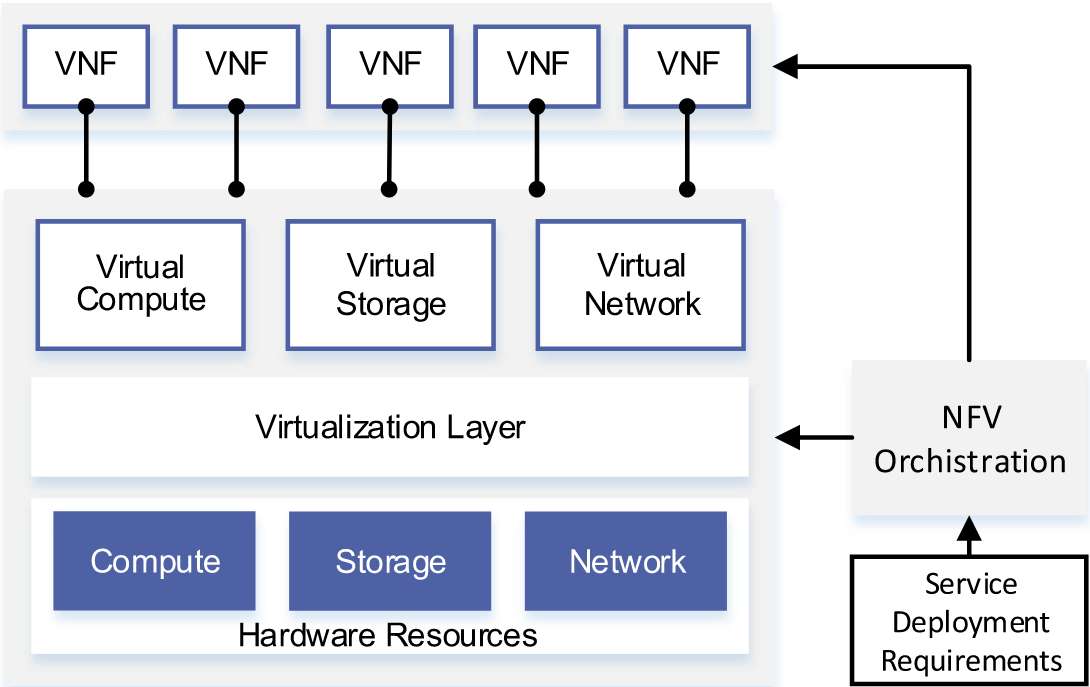
\includegraphics[width=1\linewidth]{images/nfvi.png}
	\caption{Schematic network architecture using virtual network functions \cite{li2015software}}
	\label{img:nfvi}
\end{figure}

\end{comment}



